\documentclass{bmcart}

%%%%%%%%%%%%%%%%%%%%%%%%%%%%%%%%%%%%%%%%%%%%%%
%%                                          %%
%% CARGA DE PAQUETES DE LATEX               %%
%%                                          %%
%%%%%%%%%%%%%%%%%%%%%%%%%%%%%%%%%%%%%%%%%%%%%%

%%% Load packages
\usepackage{amsthm,amsmath}
\usepackage{multicol}
\usepackage{graphicx}
\usepackage{url}
%\RequirePackage[numbers]{natbib}
%\RequirePackage{hyperref}
\usepackage[utf8]{inputenc} %unicode support
%\usepackage[applemac]{inputenc} %applemac support if unicode package fails
%\usepackage[latin1]{inputenc} %UNIX support if unicode package fails


%%%%%%%%%%%%%%%%%%%%%%%%%%%%%%%%%%%%%%%%%%%%%%
%%                                          %%
%% COMIENZO DEL DOCUMENTO                   %%
%%                                          %%
%%%%%%%%%%%%%%%%%%%%%%%%%%%%%%%%%%%%%%%%%%%%%%

\begin{document}
	
	\setlength{\parindent}{0pt} 

	\begin{frontmatter}
	
	%	\begin{fmbox}
			\dochead{Research}
			
			%%%%%%%%%%%%%%%%%%%%%%%%%%%%%%%%%%%%%%%%%%%%%%
			%% INTRODUCIR TITULO PROYECTO               %%
			%%%%%%%%%%%%%%%%%%%%%%%%%%%%%%%%%%%%%%%%%%%%%%
			
			\title{Aniridia y su relación con otras patologías}
			
			%%%%%%%%%%%%%%%%%%%%%%%%%%%%%%%%%%%%%%%%%%%%%%
			%% AUTORES. METER UNA ENTRADA AUTHOR        %%
			%% POR PERSONA                              %%
			%%%%%%%%%%%%%%%%%%%%%%%%%%%%%%%%%%%%%%%%%%%%%%
			\author[
			addressref={aff1},                   % ESTA LINEA SE COPIA IGUAL PARA CADA AUTOR
			corref={aff1},                       % ESTA LINEA SOLO DEBE TENERLA EL COORDINADOR DEL GRUPO
			email={13albertomontero@uma.es}   % VUESTRO CORREO ACTIVO
			]{\inits{A.M.}\fnm{Alberto} \snm{Montero Solera}} % inits: INICIALES DE AUTOR, fnm: NOMBRE DE AUTOR, snm: APELLIDOS DE AUTOR
			
			\author[
			  addressref={aff1},                   % ESTA LINEA SE COPIA IGUAL PARA CADA AUTOR
			  email={teresavegamar@uma.es}   % VUESTRO CORREO ACTIVO
			]{\inits{T.V.}\fnm{Teresa} \snm{Vega Martínez}} % inits: INICIALES DE AUTOR, fnm: NOMBRE DE AUTOR, snm: APELLIDOS DE AUTOR
			
			\author[
			addressref={aff1},                   % ESTA LINEA SE COPIA IGUAL PARA CADA AUTOR
			email={Alexandra.rodser.@gmail.com}   % VUESTRO CORREO ACTIVO
			]{\inits{A.R.}\fnm{Alexandra} \snm{Rodríguez Serantes}}
			
			\author[
			addressref={aff1},                   % ESTA LINEA SE COPIA IGUAL PARA CADA AUTOR
			email={Lilixia13@uma.es}   % VUESTRO CORREO ACTIVO
			]{\inits{X.L.}\fnm{Xian Li} \snm{Xia}}
			
			\vspace{10pt}
			
			
			%%%%%%%%%%%%%%%%%%%%%%%%%%%%%%%%%%%%%%%%%%%%%%
			%% AFILIACION. NO TOCAR                     %%
			%%%%%%%%%%%%%%%%%%%%%%%%%%%%%%%%%%%%%%%%%%%%%%
			
			\address[id=aff1]{%                           % unique id
			  \orgdiv{ETSI Informática},             % department, if any
			  \orgname{Universidad de Málaga},          % university, etc
			  \city{Málaga},                              % city
			  \cny{España}                                    % country
			}
		
	%	\end{fmbox}% comment this for two column layout
		
		\begin{abstractbox}
		
			\begin{abstract} % abstract
			
			%%%%%%%%%%%%%%%%%%%%%%%%%%%%%%%%%%%%%%%%%%%%%%%
			%% RESUMEN BREVE DE NO MAS DE 100 PALABRAS   %%
			%%%%%%%%%%%%%%%%%%%%%%%%%%%%%%%%%%%%%%%%%%%%%%%	
			En el presente artículo se ha profundizado en los genes asociados a la aniridia, un fenotipo relativamente desconocido que afecta al desarrollo ocular. Con objetivo de extender la información existente y mejorar la comprensión de las relaciones genotipo-fenotipo que están vinculadas a esta patología, se emplearon herramientas avanzadas que identificaron los genes más interesantes. Con estos, se exploraron sus relaciones moleculares en búsqueda de nuevas enfermedades que puedan tener conexión con la aniridia. Además, este estudio demuestra la potencialidad de los avances bioinformáticos para la investigación de procesos biológicos complejos, abriendo nuevos caminos en la biología y la medicina.
			\end{abstract}
			
			%%%%%%%%%%%%%%%%%%%%%%%%%%%%%%%%%%%%%%%%%%%%%%
			%% PALABRAS CLAVE DEL PROYECTO              %%
			%%%%%%%%%%%%%%%%%%%%%%%%%%%%%%%%%%%%%%%%%%%%%%
			
			\begin{keyword}
			\kwd{aniridia}
			\kwd{patologías}
			\kwd{iris}
			\kwd{ocular}
			\end{keyword}
		
		
		\end{abstractbox}
	
	\end{frontmatter}
	

	
	%%%%%%%%%%%%%%%%%%%%%%%%%%%%%%%%%
	%% COMIENZO DEL DOCUMENTO REAL %%
	%%%%%%%%%%%%%%%%%%%%%%%%%%%%%%%%%
	\section{Introducción}

La aniridia es un trastorno congénito del desarrollo ocular caracterizado por la
ausencia parcial o total del iris, la estructura que da color al ojo y que regula la
cantidad de luz que entra en la pupila. Esta condición, además de afectar la estética
del ojo, puede causar una serie de problemas visuales significativos, como fotofobia (sensibilidad a la luz), nistagmo (movimientos involuntarios de los ojos) y
disminución de la agudeza visual. Los individuos con aniridia a menudo presentan
malformaciones oculares asociadas, como cataratas, glaucoma (enfermedad ocular
que daña el nervio óptico, esencial para la visión) y problemas en la córnea, lo que agrava su
salud visual y afecta gravemente su calidad de vida [\cite{Landsend2021}.


No obstante, la aniridia no es solo un trastorno ocular, sino que también está
vinculada a diversas patologías sistémicas, lo que sugiere que sus mecanismos
genéticos y funcionales son complejos y multifactoriales\cite{BLACK2022389}. Por ejemplo, estudios
han mostrado que esta enfermedad puede estar asociada con el síndrome de
WAGR, una condición genética que incluye anomalías renales, tumores y problemas de desarrollo, además de la aniridia \cite{lopezrelacion}. Otros síndromes relacionados incluyen el síndrome de Gillespie, caracterizado por discapacidad intelectual, y el síndrome de Axenfeld-Rieger, que afecta tanto los ojos como otros órganos \cite{Law2011}. Estas asociaciones con condiciones sistémicas destacan la importancia de investigar en profundidad los mecanismos genéticos que subyacen
a la aniridia, así como su relación con otras patologías.


Uno de los avances más significativos en la investigación de la aniridia ha sido la 
identificación del gen \textbf{PAX6} como regulador clave del desarrollo ocular. PAX6 es un factor de transcripción que juega un papel crucial en
la diferenciación de diversas estructuras oculares, regulando la expresión de otros genes esenciales para este proceso \cite{robles_lopez_2012}. Las mutaciones en PAX6 han sido vinculadas
no solo con la aniridia, sino también con otras anomalías oculares como la displasia corneal (alteración en el desarrollo o estructura de la córnea) y el glaucoma
congénito  \cite{CalvaoPires2014}. Sin embargo, para entender completamente la heterogeneidad clínica de la aniridia, es fundamental analizar cómo interactúa
PAX6 con otros genes en redes genéticas más amplias.


Además de PAX6, varios genes han demostrado ser importantes para entender la
complejidad de la aniridia y sus trastornos asociados, entre ellos \textbf{FOXC1}, \textbf{WT1},
\textbf{FOXE3} y \textbf{PITX2}.

Las mutaciones en \textbf{FOXC1} \cite{NCBIGeneFOXC1}  están asociadas con el síndrome de Axenfeld-Rieger,
un trastorno que incluye glaucoma y otras anomalías oculares \cite{Reis2023}. Este gen codifica un factor de transcripción que, al igual que PAX6, regula
el desarrollo del ojo, y su interacción con otros genes es clave para comprender las
manifestaciones clínicas variadas que se presentan en estos pacientes. La integración
de FOXC1 en los análisis de redes génicas permite explorar cómo las vías de desarrollo ocular pueden estar interconectadas con otras rutas reguladoras sistémica.


Otro gen relevante es \textbf{WT1}, conocido por su papel en el desarrollo renal y la formación de tumores. Las mutaciones en WT1 están vinculadas al síndrome de
WAGR. La investigación sobre WT1 desde una perspectiva de biología de sistemas permite investigar cómo los defectos en los programas de desarrollo que afectan
tanto a los ojos como a otros órganos pueden estar mediadas por la interacción de redes génicas compartidas \cite{Pelletier1991}.

\textbf{FOXE3} es un gen sin intrones que pertenece a la familia de factores de transcripción "Forkhead", que regulan la expresión de otros genes específicos de tejido cruciales para la diferenciación y desarrollo. La proteína que se codifica desempeña un importante papel en la formación del cristalino en vertebrados, siendo un factor de transcripción específico. Además, las mutaciones de este gen están relacionadas con disgenesia mesenquimal (desarrollo incompleto del tejido mesenquimático) del segmento anterior del ojo y afaquia primaria congénita (ausencia del cristalino).


Finalmente, el gen \textbf{PITX2} está involucrado en la morfogénesis craneofacial y cardiovascular. Las mutaciones en este gen están asociadas con el sóndrome de Axenfeld-Rieger, afectando no solo a los ojos, sino también al desarrollo de órganos internos, debido a su rol en la simetría del desarrollo\cite{French2021}. Desde la
perspectiva de la biología de sistemas, PITX2 representa un nodo crítico dentro de redes regulatorias que conectan el desarrollo de múltiples órganos, lo que resalta cómo las disfunciones en un solo gen pueden dar lugar a manifestaciones clínicas en varios sistemas.


El objetivo de este trabajo es examinar las patologías asociadas al fenotipo de la aniridia desde el punto de vista de la biología de sistemas, enfocándonos en los genes que tienen una relación funcional con \textbf{PAX6}. A través de la identificación de genes asociados y el análisis de redes génicas y moleculares mediante técnicas como la creación de clusters\cite{ben1999clustering} y el análisis de redes funcionales \cite{FloresCamacho2009}, se tratará de avanzar en la comprensión de cómo las interacciones entre estos genes contribuyen a la presentación clínica de la aniridia
y sus trastornos relacionados. Este enfoque no solo amplía nuestro conocimiento sobre la aniridia, sino que también ofrece información valiosa sobre los mecanismos
patológicos que interconectan diversas condiciones sistémicas.


	\section{Materiales y métodos}

En esta sección serán expuestos las diferentes herramientas y métodos utilizados para llevar a cabo el proyecto, así como los resultados obtenidos con cada una de ellas.

\subsection{Materiales}
\subsubsection{Human Phenotype Ontology}

La \textbf{Human Phenotype Ontology (HPO)} es un proyecto que desarrolla un vocabulario estandarizado y jerárquico para describir fenotipos humanos, con el objetivo de apoyar el diagnóstico y la investigación de enfermedades genéticas. Además de definir y organizar características fenotípicas específicas, la HPO permite identificar los genes y variantes genéticas asociadas a cada fenotipo, de esta manera facilita el análisis de correlaciones genotipo-fenotipo a los usuarios.

\subsubsection{STRING}

\textbf{STRING} es una base de datos que integra distintas fuentes de información y que además permite analizar y visualizar interacciones entre proteínas y genes. Pueden ser de dos tipos: interacciones físicas o interacciones funcionales. Las interacciones físicas permiten identificar compatibilidades y relaciones, mientras que las funcionales determinan si dos o más proteínas son compatibles aún sin tener interacción directa. Así pues, se pueden realizar perfiles filogenéticos y conocer genes con patrones similares, además de aportar información sobre patrones moleculares, mapas bioquímicos y mejorar la compresión de los sistemas biológicos.

\subsubsection{Python}
\textbf{Python} es uno de los lenguajes de programación más usados del mundo. Se trata de un lenguaje de alto nivel con una sintaxis sencilla y fácil de entender que dispone de multitud de paquetes de código abierto. Se caracteriza por ser interpretado, es decir, no se requiere de compilación previa a instrucciones de lenguaje máquina ya que se emplea un entorno o intérprete para ejecutar el código. La versión utilizada en este proyecto es ?.

\subsubsection{R}
\textbf{R} es otro de los lenguajes de programación más importantes en el campo de la estadística. Es un entorno de software libre y también es un lenguaje interpretado. A diferencia de otros softwares de análisis de datos, R tiene un entorno completamente integrado y coherente. Proporciona una amplia gama de técnicas estadísticas y gráficas. La versión utilizada en este proyecto es ?.

\subsubsection{iGraph}
\textbf{iGraph} es una biblioteca de código abierto utilizada para el análisis y visualización de redes complejas. Es una herramienta muy útil para el estudio de los sistemas biológicos ya que estos están compuestos por genes, moléculas, proteínas, etc, que interactúan formando grafos complejos de analizar a simple vista. Está implementado en C, aunque también puede ser utilizado en otros lenguajes como R y Python. 

Esta herramienta presenta muchas ventajas, entre las que destacamos: la integración de todo tipo de datos ómicos, la visualización de datos de forma interactiva, mejora la comprensión de las relaciones entre las distintas biomoléculas del sistema, permite la identificación de nodos clave en la red biológica, facilita el descubrimiento de grupos funcionales de genes o proteínas y predice cómo ciertas modificaciones podrían perturbar los sistemas.

\subsubsection{Pandas}
\textbf{Pandas} se trata de una popular librería de Python de código abierto muy necesaria para el ámbito de Data Science y Machine Learning. Proporciona unas estructuras poderosas y flexibles implementando todas las herramientas necesarias para el análisis de datos, ya que permite la carga, modelado, análisis, manipulación y preparación de datos.

\subsubsection{Algoritmos de clusterización}
En el presente proyecto, uno de los objetivos es la identificación de patrones entre los distintos genes asociados al fenotipo de la aniridia. Para ello, es necesario el agrupamiento de aquellas biomoléculas con mayor similitud dentro nuestra red biológica, así que se aplicarán algoritmos nos permitan detectar estructuras sin necesidad de tener conocimiento previo. Vamos a hablar de los algoritmos de Givan-Newman, de optimización voraz, de propagación de etiquetas y de Louvain.

Primero, tenemos el \textbf{algoritmo de Givan-Newman}, que es uno de los métodos más utilizados para la detección de comunidades dentro de sistemas complejos de datos. Su funcionamiento se basa en eliminar progresivamente aquellos enlaces que conectan grupos de nodos con mayor densidad dentro de la red, para visualizar finalmente subgrafos desconectados que representan las comunidades.

Por otra parte, el \textbf{algoritmo de optimización voraz} es un algoritmo que dado un problema, elige aquellas decisiones localmente óptimas con el propósito de encontrar la solución más óptima globalmente. A medida que va tomando unas decisiones, el algoritmo no reconsidera ningún paso ya realizado.

Además, el \textbf{algoritmo de propagación de etiquetas} es una técnica que nos permite encontrar comunidades dentro del sistema velozmente. El funcionamiento se basa en la asignación de etiquetas a nodos, que en cada iteración se van propagando por la red y converge finalmente cuando cada nodo posee la etiqueta perteceneciente a su vecino más cercano. Una de las ventajas de este algoritmo es que no es necesaria la predefinición de un número de clústers.

Por último, el \textbf{algoritmo de Louvain} se basa en el concepto de modularidad, es decir, tiene como objetivo maximizar el número de aristas dentro de una comunidad y minimizar el número de relaciones entre distintas comunidades. Este algoritmo es muy recomendable para sistemas biológicos muy amplios, ya que se obtienen comunidades compactas y bien definidas.

\subsubsection{Otras librerías empleadas}

\subsubsection{Software empleado para la generación de diagramas}

\subsubsection{GitHub?}

\vspace{3pt}
\subsection{Métodos}
BORRADOR:
*OPCIÓN 1*
Para realizar este estudio, el primer paso que se llevó a cabo fue la obtención de los genes relacionados con el fenotipo. Los descargamos de la página Human Phenotype Ontology mediante la introducción del ID del fenotipo, en nuestro caso "HP:0000526". Una vez obtenidos los genes, realizamos una red de interacción de los genes asociados a nuestro fenotipo mediante la herramienta STRINGDB.

A continuación, se muestran los pasos llevados a cabo para obtener una red de interacción de los genes de un fenotipo concreto:

\begin{itemize}
	\item Visitamos la página de STRING
	\item Seleccionamos la opción para intnroducir múltiples proteínas
	\item Introducimos solo los nombres de los genes descargados de Human Phenotype Ontology.
	\item Especificamos la especie, en este caso, Homo sapiens.
	\item STRING generará una red de interacciones, mostrando conexiones basadas en interacciones experimentales, predicciones y bases de datos de coexpresión.
	\item Se guarda como imagen la red obtenida.
\end{itemize}

Entre los objetivos del uso de STRING están visualizar las interacciones proteicas conocidas y predichas, identificar posibles proteínas clave o "hubs" dentro de la red y evaluar la conectividad y la funcionalidad de los genes en el contexto del fenotipo elegido.

Tras introducir el nombre de todos los genes asociados a nuestro fenotipo obtuvimos la siguiente red de interacciones:

\newpage

\begin{figure}[h] % [h] indica que queremos la imagen aquí, en la posición actual
	\centering
	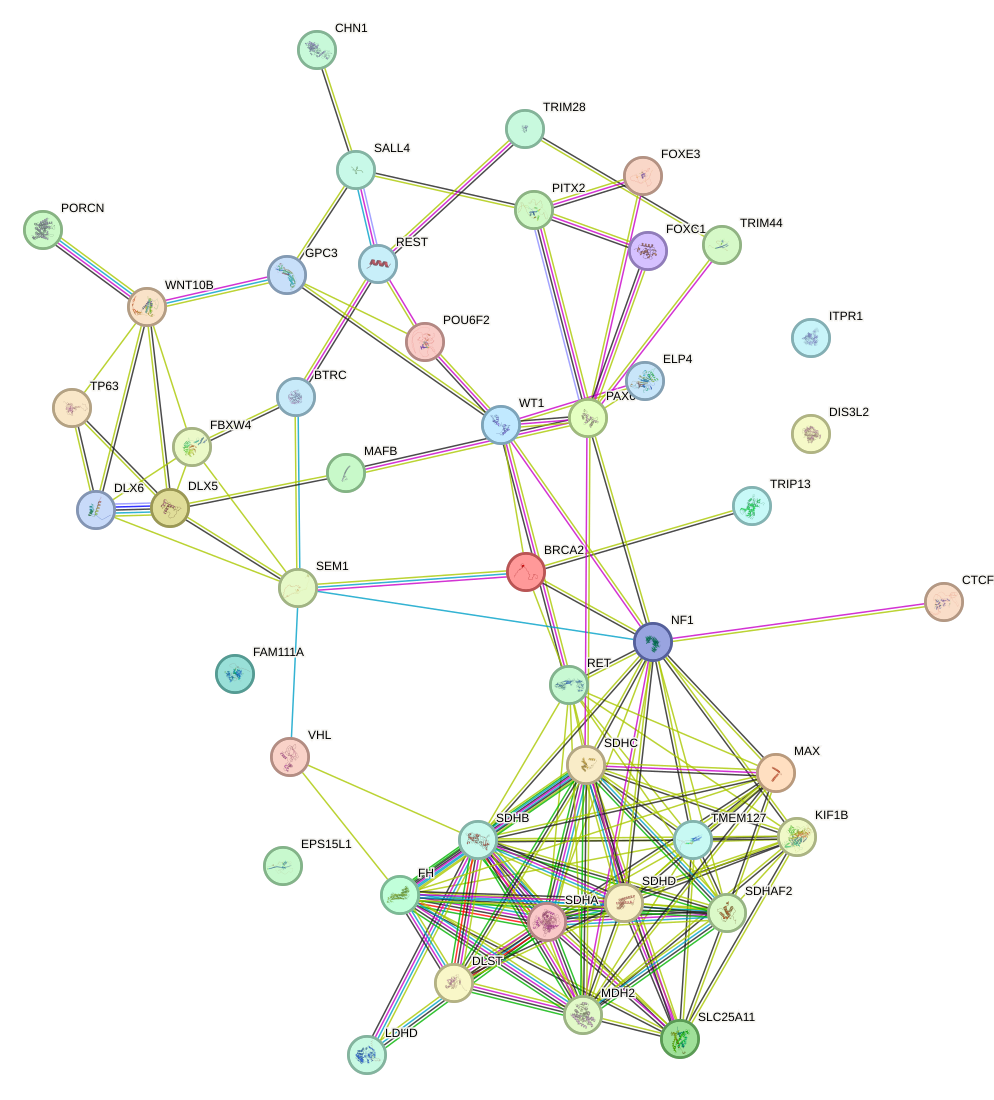
\includegraphics[width=1\textwidth]{figures/red_interaccion_aniridia.png} % Especifica la ruta y el tamaño
	\caption{Red de interacción con los genes asociados al fenotipo HP:0000526} % Agrega una leyenda si deseas
	\label{fig:mi-imagen} % Etiqueta para referenciar la imagen en el texto
\end{figure}

*OPCIÓN 2*
Para la identificación de genes asociados a la aniridia, implementamos una función en Python que hace uso de la API de Human Phenotype Ontology (HPO). Esta función recibe como parámetro el código HPO del fenotipo de interés, en este caso la aniridia, cuyo código es HP:0000526. Con este código realiza una solicitud GET a la API de HPO para recuperar información sobre los genes asociados. Si la respuesta es satisfactoria (código de estado 200), extrae y devuelve la lista de genes vinculados al fenotipo. En caso contrario, se imprime un mensaje de error y se devuelve una lista vacía.

Posteriormente, construimos una URL utilizando los símbolos de los genes obtenidos, para hacer una solicitud GET a la API de StringDB. Esta API proporciona datos sobre interacciones de proteínas. La solicitud devuelve una red de interacciones de proteínas, la cual almacenamos en la imagen .
También analizamos y filtramos los resultados de enriquecimiento en categorías relevantes. Las búsquedas específicas en estos resultados de enfermedades y genes se realizan mediante palabras clave y patrones relevantes, y los resultados se guardan en archivos CSV para facilitar su análisis posterior.

Finalmente, descargamos la red de interacciones en formato TSV usando otra solicitud GET a la API de StringDB. Si la descarga es exitosa, el archivo se guarda con el nombre de archivo especificado o, en caso contrario, con el nombre predeterminado reddescargada.tsv. Ante cualquier error en la descarga, se imprime un mensaje de advertencia.

Al cargar el archivo TSV descargado, seleccionamos las columnas de nombres preferidos y eliminamos las filas duplicadas. Estos datos se guardan en un archivo de texto llamado genesigraph.txt, que contiene únicamente los nombres de los genes relevantes para un análisis adicional de la red biológica.

\subsubsection{Flujo de trabajo}



	\section{Resultados}

\subsection{Red de interacciones inicial}


\begin{figure}[h] % [h] indica que queremos la imagen aquí, en la posición actual
	\centering
	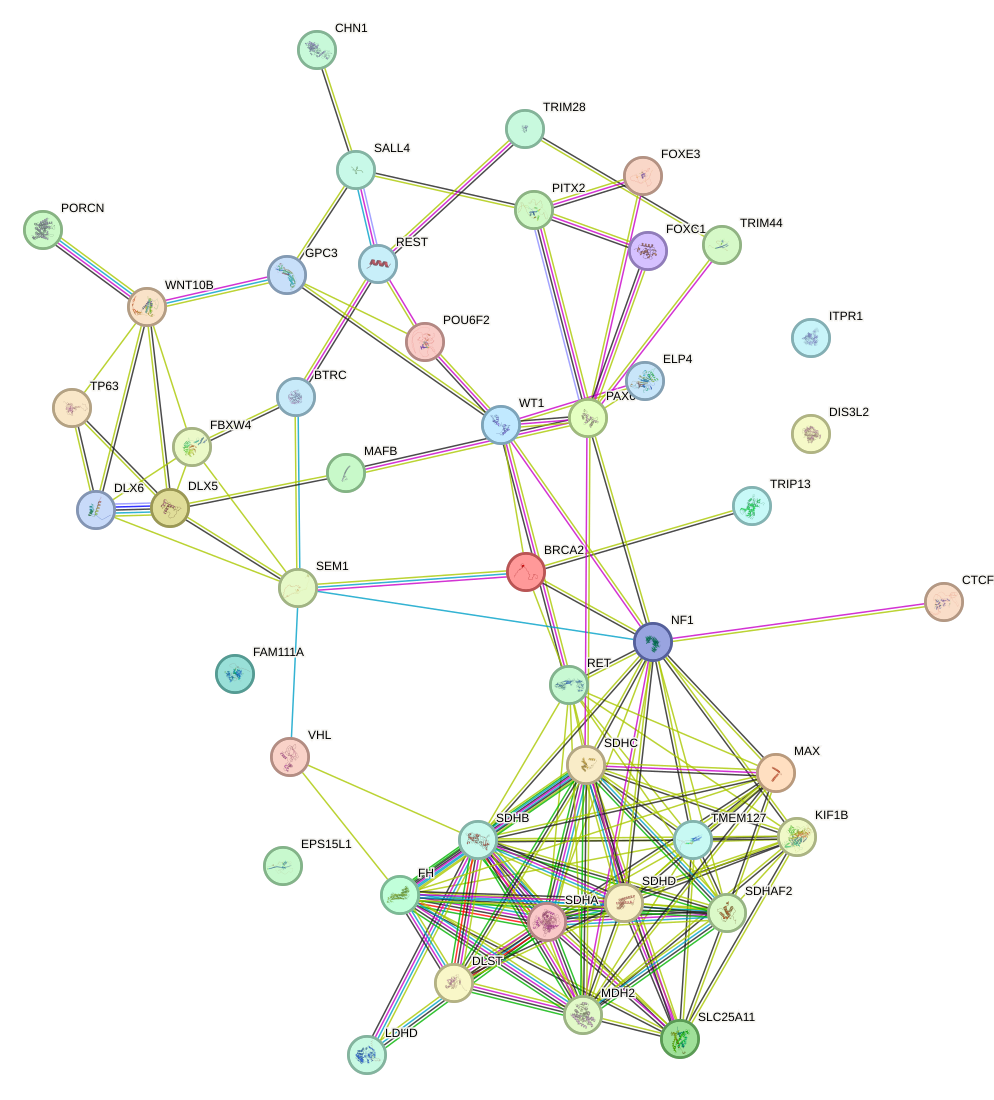
\includegraphics[width=1\textwidth]{figures/red_interaccion_aniridia.png} % Especifica la ruta y el tamaño
	\caption{Red de interacción con los genes asociados al fenotipo HP:0000526} % Agrega una leyenda si deseas
	\label{fig:mi-imagen} % Etiqueta para referenciar la imagen en el texto
\end{figure}

\subsection{Propagación de la red}

A partir de los genes semilla WNT10B, WT1, SEM1, PAX6, y NF1, se generó una red de interacciones proteína-proteína (PPI) utilizando datos de STRINGdb. Se estableció un umbral de puntaje de interacción de 700 para incluir únicamente conexiones de alta confianza. La red inicial centrada en los genes semilla fue posteriormente expandida mediante el algoritmo DIAMOnD, incluyendo 200 nodos adicionales que se encuentran altamente conectados con los genes semilla y entre sí.

La red generada señala importantes interacciones entre los genes semilla y otros desconocidos (como la relación WNT10B - TGFB2), lo cual permite continuar el estudio hacia el objetivo del artículo.

\subsection{Clustering}

\begin{figure}[h] % [h] indica que queremos la imagen aquí, en la posición actual
	\centering
	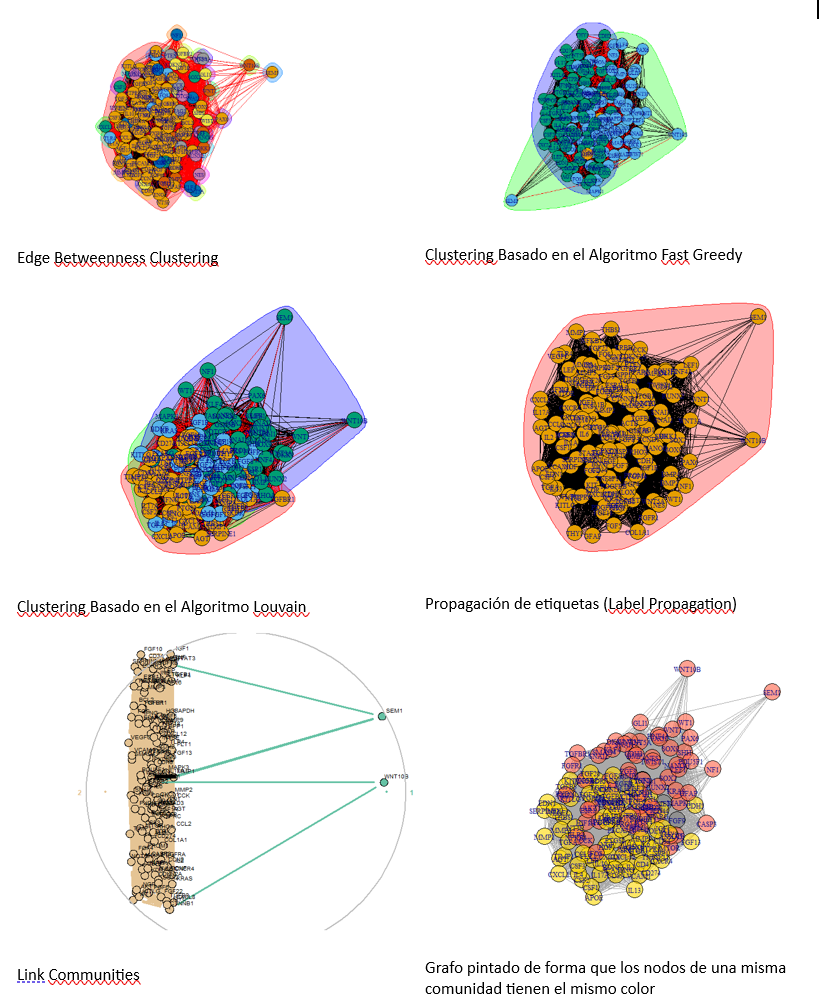
\includegraphics[width=1\textwidth]{figures/toda_figuras_clustering.png}
	\caption{Figuras obtenidas al aplicar clustering con distintos métodos}
	\label{clustering}
\end{figure}

Principalmente el estudio de los resultados se centrará en los genes semilla (WNT10B, WT1, SEM1, PAX6, NF1). En común, se puede observar que SEM1 aparece en varisa posiciones destacadas en los grafos; WT1 y PAX6 están en regiones densas (centrales) de las comunidades, lo que infica que tienen muchas conexiones internas; y NF1 se sitúa en los bordes de las comunidades, por lo que podría actuar como puente entre diferentes comunidades; y WNT10B también es central en algunas comunidades.




\subsection{Enriquecimiento y combinación de fenotipos}

Al realizar un análisis de enriquecimiento considerando la categoría “Process” generamos un archivo que nos permite comprender en qué procesos biológicos clave están involucrados los genes del cluster seleccionado. Esto ayuda a identificar rutas metabólicas, mecanismos celulares y funciones moleculares que pueden estar asociados con el fenotipo de interés.

Por otra parte, realizar el enriquecimiento funcional considerando categoría “HPO” es crucial para identificar cómo los genes analizados están asociados con características fenotípicas específicas, especialmente aquellas relacionadas con enfermedades humanas. 
Por último, combinar los fenotipos resultantes del enriquecimiento y los asociados a las enfermedades asociadas a nuestro fenotipo permite confirmar si los términos fenotípicos enriquecidos en los clusters tienen una relación directa con las enfermedades previamente identificadas. Si hay coincidencias, esto valida que los genes analizados están realmente relacionados con el fenotipo de interés.

Además, el establecer identificaciones entre las relaciones genotipo-fenotipo ayuda a establecer conexiones concretas entre los genes y las manifestaciones clínicas observadas en pacientes. Esto es especialmente útil para comprender cómo los genes influyen en el desarrollo de ciertas enfermedades o características clínicas.

Finalmente, podemos ver que 284 fenotipos de los 668 obtenidos tras el enriquecimiento están relacionados con enfermedades relacionadas con nuestro fenotipo a estudiar. Este resultado sugiere que el análisis de enriquecimiento funcional está capturando información biológica y clínica relevante. La conexión entre los fenotipos obtenidos y las enfermedades relacionadas con la aniridia valida que los genes analizados están efectivamente implicados en procesos relacionados con el fenotipo de interés. Este hallazgo podría abrir la puerta a la identificación de procesos centrales o vías moleculares críticas en estas enfermedades.
Por otra parte,  los fenotipos compartidos pueden ayudar a priorizar genes o grupos de genes específicos para estudios adicionales. Estos genes podrían ser considerados como potenciales biomarcadores o dianas terapéuticas para tratar tanto la aniridia como las enfermedades relacionadas.
Los fenotipos no relacionados también son interesantes, ya que podrían reflejar aspectos únicos del fenotipo de interés o nuevas áreas de estudio.






	\section{Discusión}

El análisis de la \textbf{aniridia} como fenotipo central permitió identificar múltiples asociaciones relevantes con enfermedades genéticas descritas en bases de datos especializadas como OMIM y Orphanet. En los datos analizados, se observa que la aniridia (HPO:0000526) está presente en una amplia variedad de condiciones, reflejando su relevancia clínica y biológica. Estas incluyen, entre otras, *Axenfeld-Rieger syndrome, type 1* (OMIM:180500), *D-lactic aciduria with susceptibility to gout* (OMIM:245450), *Nephroblastoma* (ORPHA:654) y *Chromosome 11p13 deletion syndrome, distal* (OMIM:616902). Cada una de estas enfermedades aporta perspectivas complementarias sobre los mecanismos genéticos y moleculares asociados a la aniridia.

El gen \textit{PAX6}, ampliamente reconocido como un regulador maestro en el desarrollo ocular, surge como un elemento central en el análisis de redes de interacción genética. Este gen no solo está directamente relacionado con la aniridia, sino que también actúa como un nodo crítico en las redes moleculares que controlan procesos como la diferenciación de tejidos oculares, el desarrollo neuronal y la señalización celular. Adicionalmente, genes como \textit{WT1} y \textit{NF1}, identificados en las redes extendidas generadas, refuerzan la idea de que la aniridia no es un fenotipo aislado, sino que forma parte de una red compleja de interacciones genéticas con implicaciones multisistémicas.

La diversidad de enfermedades asociadas a la aniridia destaca la importancia de abordar este fenotipo desde una perspectiva interdisciplinaria. Por ejemplo, en condiciones como el *Nephroblastoma* y el *Chromosome 11p13 deletion syndrome*, la aniridia es acompañada de fenotipos adicionales como hipertensión, hemihipertrofia y retraso en el desarrollo psicomotor. Estas asociaciones subrayan la necesidad de considerar no solo los fenotipos primarios, sino también los secundarios o relacionados, para realizar diagnósticos más precisos.

El análisis funcional de los fenotipos asociados también resalta que un número significativo de enfermedades relacionadas con la aniridia involucran procesos moleculares como la regulación del desarrollo embrionario, la señalización del factor de crecimiento transformante beta (TGF-β), y la reparación del ADN. Esto sugiere que los mecanismos subyacentes a la aniridia podrían incluir disfunciones en rutas moleculares comunes que contribuyen tanto a defectos estructurales como a susceptibilidades a enfermedades malignas.

Aunque el presente análisis se centra en asociaciones conocidas y documentadas en bases de datos como HPO, OMIM y Orphanet, es fundamental reconocer las limitaciones de estas fuentes. Las interacciones gen-fenotipo podrían estar infraestimadas debido a la falta de datos en poblaciones específicas o por la subrepresentación de variantes genéticas raras en estas bases de datos. Por lo tanto, futuros estudios deberían incluir enfoques complementarios, como el análisis transcriptómico y proteómico en tejidos afectados, para identificar patrones moleculares específicos de la aniridia.

En conclusión, la \textbf{aniridia} no solo es un marcador clínico de enfermedades genéticas específicas, sino también una ventana a la comprensión de redes moleculares más amplias que subyacen a defectos del desarrollo y condiciones multisistémicas. La integración de herramientas bioinformáticas, redes moleculares y datos clínicos puede mejorar significativamente el diagnóstico y manejo de estas enfermedades, abriendo además oportunidades para desarrollar terapias dirigidas basadas en los mecanismos subyacentes identificados.

	\section{Conclusiones}

El enfoque utilizado en este estudio demuestra el potencial de las herramientas bioinformáticas para desentrañar la complejidad de fenotipos clínicos como la aniridia. A través de una combinación de análisis de red, clustering y enriquecimiento funcional, hemos identificado genes clave y procesos moleculares relacionados con los fenotipos de la enfermedad. Este trabajo no solo confirma la validez del modelo aplicado, sino que también destaca nuevas áreas de investigación y posibles aplicaciones clínicas, contribuyendo al conocimiento de la base genética y molecular de la aniridia.
	
	
	%%%%%%%%%%%%%%%%%%%%%%%%%%%%%%%%%%%%%%%%%%%%%%
	%% OTRA INFORMACIÓN                         %%
	%%%%%%%%%%%%%%%%%%%%%%%%%%%%%%%%%%%%%%%%%%%%%%
	
	\begin{backmatter}
	
		\section*{Abreviaciones}%% if any
			Indicar lista de abreviaciones mostrando cada acrónimo a que corresponde
		
		\section*{Disponibilidad de datos y materiales}%% if any
			\url{https://github.com/monteero13/project_template.git}
		
		\section*{Contribución de los autores}
			Usando las iniciales que habéis definido al comienzo del documento, debeis indicar la contribución al proyecto en el estilo:
			J.E : Encargado del análisis de coexpresión con R, escritura de resultados; J.R.S : modelado de red con python y automatizado del código, escritura de métodos; ...
			OJO: que sea realista con los registros que hay en vuestros repositorios de github. 
		
		
		%%%%%%%%%%%%%%%%%%%%%%%%%%%%%%%%%%%%%%%%%%%%%%%%%%%%%%%%%%%%%%%%%%%%%%%%%%%%%%%%%%%%%%%%
		%% BIBLIOGRAFIA: no teneis que tocar nada, solo sustituir el archivo bibliography.bib %%
		%% por el que hayais generado vosotros                                                %%
		%%%%%%%%%%%%%%%%%%%%%%%%%%%%%%%%%%%%%%%%%%%%%%%%%%%%%%%%%%%%%%%%%%%%%%%%%%%%%%%%%%%%%%%%
		
		\bibliographystyle{bmc-mathphys} % Style BST file (bmc-mathphys, vancouver, spbasic).
		\bibliography{bibliography}      % Bibliography file (usually '*.bib' )
	
	\end{backmatter}
\end{document}
